We present the experiments and results used to evaluate \scheme{} in this section.

\subsection{Experimental Setup} \label{sec:eval-setup}
We conducted three sets of experiments.
First, we evaluated the impact of \jscheme{} and \bscheme{} on average packet network latency with varying injection rates using the Garnet~\cite{agarwal2009garnet} simulator.
Second, we measured the performance overhead of both schemes on real applications from the PARSEC~\cite{bienia2008parsec} and Rodinia~v3.0~\cite{che2009rodinia} benchmark suites using the Gem5~\cite{binkert2011gem5} simulator.
Finally, we conducted sensitivity studies to identify optimal design parameters.

We evaluated five policies summarized in Table~\ref{tab:policies}.
All performance results are normalized to \basescheme{} (the insecure baseline without bypass).
When comparing against \basebscheme{}, we state so explicitly.
We used a 64-core machine modeled as an $8\times8$ 2D mesh with a 32~kB L1 cache per core and a 2~MB distributed LLC.
For Rodinia applications, we executed 1B instructions in the region of interest where threads are spawned by the OpenMP library.
For PARSEC applications, we executed 1B instructions or until the end of the marked region of interest.
We treat all load requests arriving at the LLC as Security Sensitive instructions to model the worst-case overhead of \scheme{}.

\begin{table}[t]
    \centering
    \begin{tabular}{|p{0.3\linewidth}|p{0.6\linewidth}|}
        \hline \hline
        \textbf{Policy} & \textbf{Description} 
        \\ \hline
        \basescheme{} 
        & Insecure $8\times8$ 2D mesh baseline 
        \\ \hline
        \basebscheme{} 
        & Bypass network on top of \basescheme{} following~\cite{perez2019smart++}, without security enforcement \\ 
        \hline
        \jscheme{} 
        & \basescheme{} extended with a delay queue at each NI; delays all Security Sensitive LLC hits to $T_{worst}$ \\ 
        \hline
        \bscheme{} 
        & \basescheme{} extended with bypass and delay; enforces $T_{low}$ for all Security Sensitive LLC hits \\ 
        \hline
        \rscheme{}
        & \basescheme{} extended with bypass and delay; draws a random target from $[T_{floor}, T_{low}]$ per access instead of enforcing the fixed $T_{low}$ \\
        \hline
    \end{tabular}
    \caption{The five evaluated policies. 
    All results are normalized to \basescheme{}.}
    \label{tab:policies}
\end{table}

\subsection{Average Packet Network Latency} \label{sec:avg-latency}
We used the Garnet simulator to measure average packet latency at varying injection rates.
Figure~\ref{fig:overall_packet_network_latency} shows the results.
\bscheme{} performs comparably to \basescheme{} across all injection rates: using bypass paths for Security Sensitive loads does not adversely affect overall average packet latency.
In contrast, \jscheme{} causes the network to saturate earlier than \basescheme{} at higher injection rates, due to the delay queue increasing congestion in the network.

\basebscheme{} and \bscheme{} are visually identical in this figure: bypass alone already meets the target latency, so the delay-convergence check has nothing left to do.
\jscheme{} and \basescheme{} converge too, but only past the saturation knee, once padding no longer fires.
Below saturation the two remain distinguishable, just not at a scale visible on this axis.

\begin{figure}[t]
    \centering
    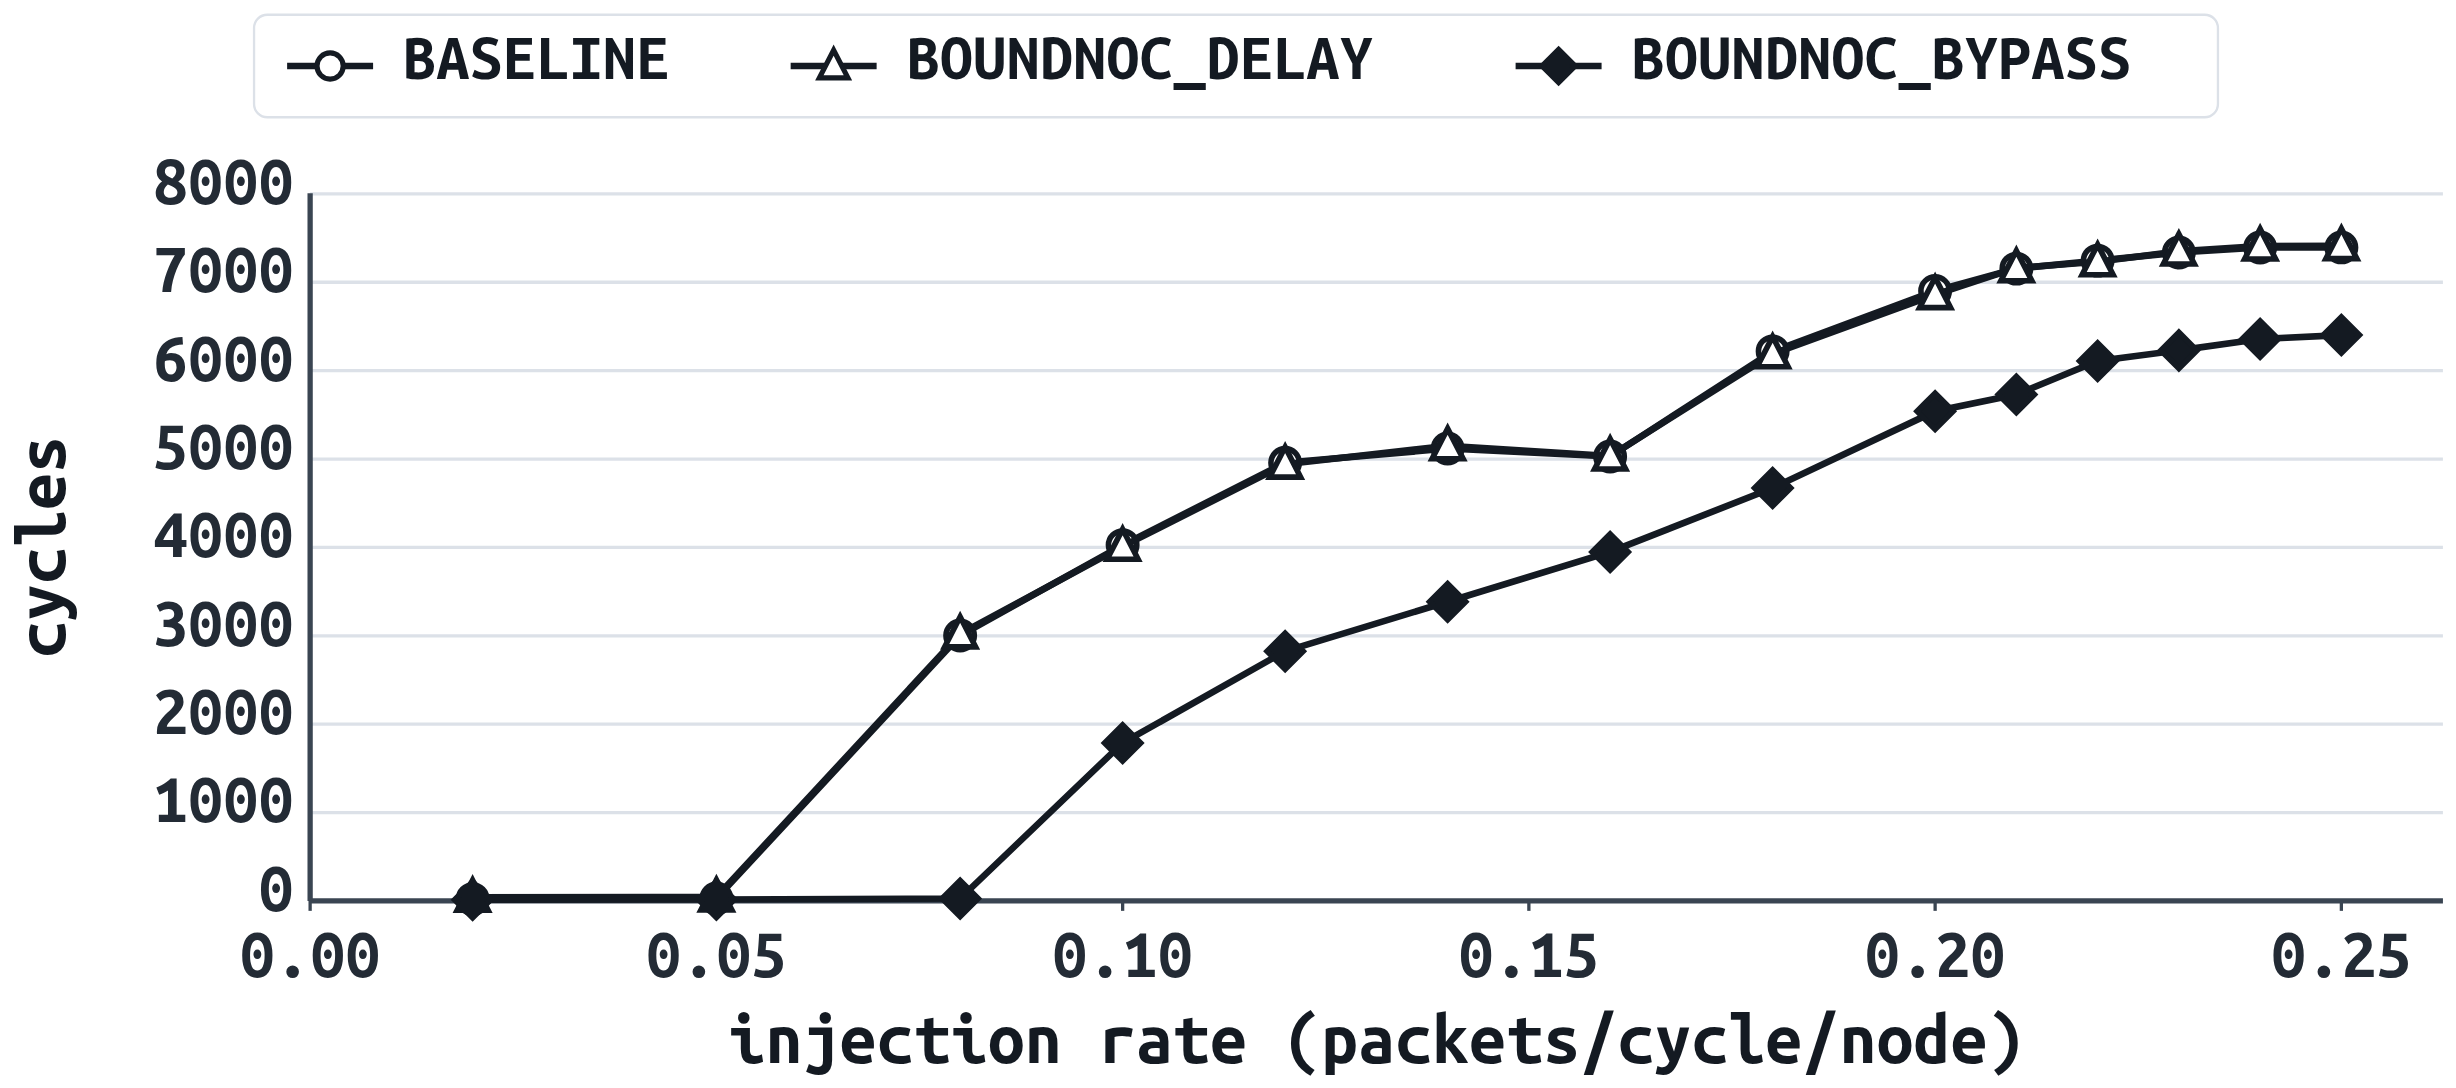
\includegraphics[width=\linewidth]{figs_new/boundnoc_injection_rate_sweep.png}
    %{figs/overall_packet_network_latency.pdf}
    \caption{Average packet latency vs.\ injection rate for \basescheme{}, \basebscheme{}, \jscheme{}, and \bscheme{}, using uniform-random synthetic traffic on an $8\times8$ mesh (Garnet\_standalone).}
    \label{fig:overall_packet_network_latency}
\end{figure}

\subsection{Impact on Secure Load Latency} \label{sec:secure-ld-latency}
We evaluate the impact of each policy on the round-trip latency of Security Sensitive loads using both synthetic and real workloads.

\subsubsection{Synthetic Workload} 
Figure~\ref{fig:impact-on-latency-syn} shows the round-trip latency of Security Sensitive loads at varying injection rates using the Garnet simulator.
In the baseline, near-tile and far-tile accesses are clearly distinguishable.
Both \jscheme{} and \bscheme{} eliminate this distinction, making near- and far-tile latencies indistinguishable from the the perspective of the attacker.
However, \jscheme{} incurs a significantly higher absolute latency than \bscheme{}, since all accesses are delayed to $T_{worst}$ rather than $T_{low}$.

\subsubsection{Real Workload}
Figure~\ref{fig:impact-on-latency} (\S\ref{sec-security-real}) confirms that \jscheme{} and \bscheme{} both produce overlapping latency distributions for the closest and farthest node pairs on leukocyte, a real application.

\subsection{Performance Overhead} \label{sec:perf-overhead}

\begin{figure*}[t]
\centering
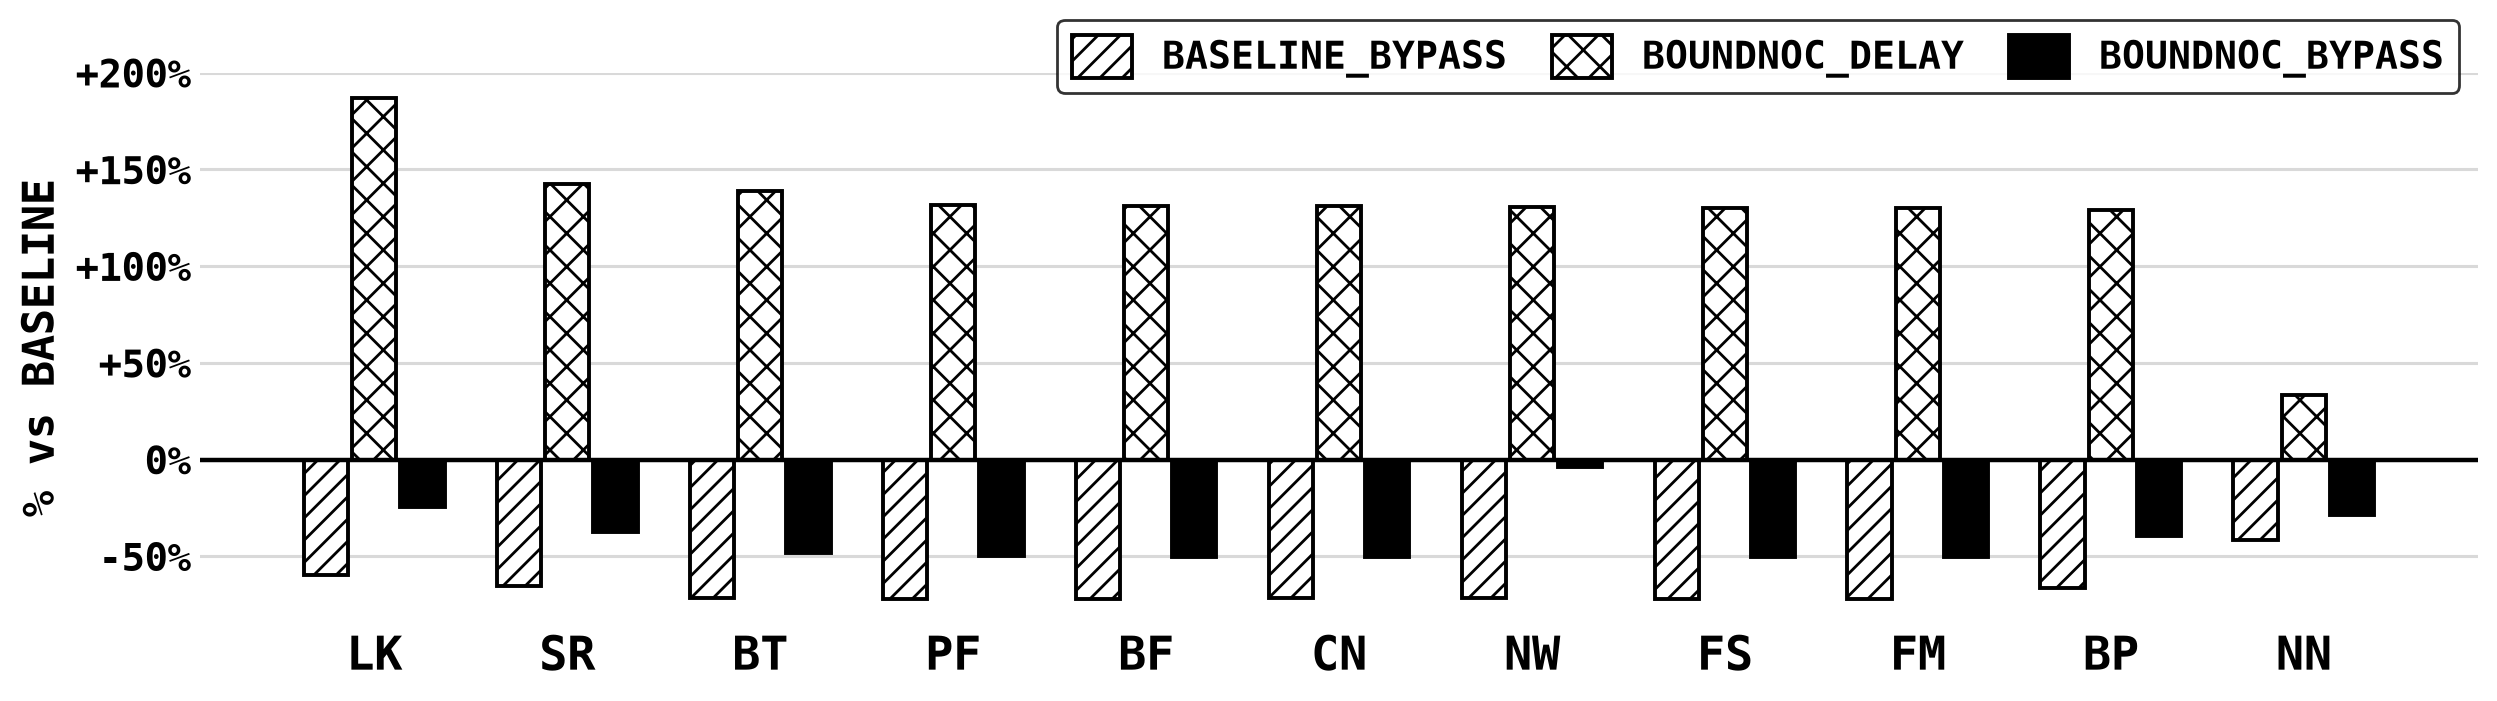
\includegraphics[width=\linewidth]{figs_new/boundnoc_latency_pctdelta.png}
%{figs/performance-overhead.pdf}
\caption{Performance overhead of \jscheme{} and \bscheme{} on PARSEC~\cite{bienia2008parsec} and Rodinia~\cite{che2009rodinia} benchmarks, normalized to \basescheme{}.
Shorthand described in the Appendix.}
\label{fig:performance-overhead}
\end{figure*}

Figure~\ref{fig:performance-overhead} shows the performance overhead of all four policies.
\jscheme{} incurs $0.53\%$--$15.0\%$ overhead over \basescheme{}, with a geomean of $7.24\%$ across all applications.
Compared to the insecure \basebscheme{}, \jscheme{} overhead is $11.94\%$ and \bscheme{} overhead is $1.96\%$.

Figure~\ref{fig:bypass-count} shows that the bypass packet count of \bscheme{} matches that of \basebscheme{} closely in every benchmark, differing by at most $2\%$.
\bscheme{} uses the same bypass decision as \basebscheme{}; the only added cost is the delay needed to pad each response up to $T_{low}$.
This is why the overhead of \bscheme{} over \basebscheme{} stays small ($1.96\%$ geomean) across every application we tested.

\begin{figure*}[t]
\centering
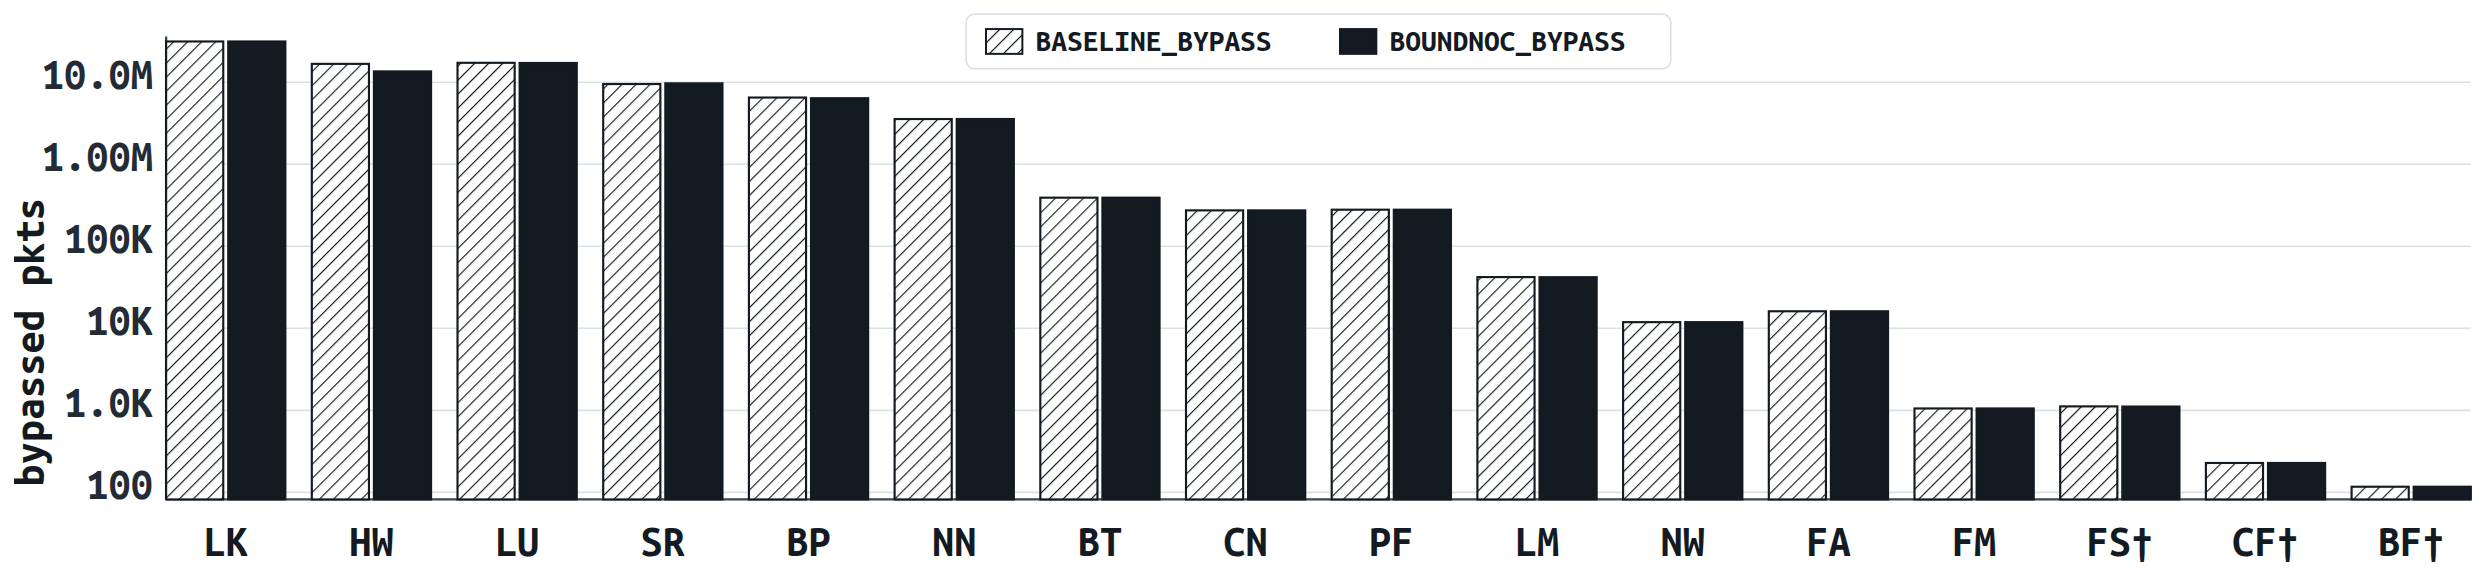
\includegraphics[width=\linewidth]{figs_new/boundnoc_bypass_count.png}
%{figs/bypass-count.pdf}
\caption{Total bypass packet count for \basebscheme{} and \bscheme{} using PARSEC~\cite{bienia2008parsec} and Rodinia~\cite{che2009rodinia} benchmarks.}
\label{fig:bypass-count}
\end{figure*}

%In some applications, \bscheme{} does not improve over \basescheme{}.
%For example, x264 incurs $4\%$ overhead under \bscheme{}.
%In x264, \bscheme{} causes certain threads to execute more instructions before the 1B-instruction termination condition is met on any thread, increasing the measured execution time relative to baseline.

\subsection{Impact on Delay Amount} \label{sec:delay-amount}
Figure~\ref{fig:delay-amount} shows the total delay cycles accumulated in the delay queue for PARSEC applications.
\jscheme{} forces all Security Sensitive packets to wait in the delay queue until $T_{worst}$, resulting in high total delay.
\bscheme{} delays only packets that arrive earlier than $T_{low}$, substantially reducing total delay cycles and the associated performance overhead.

\begin{figure*}
    \centering
    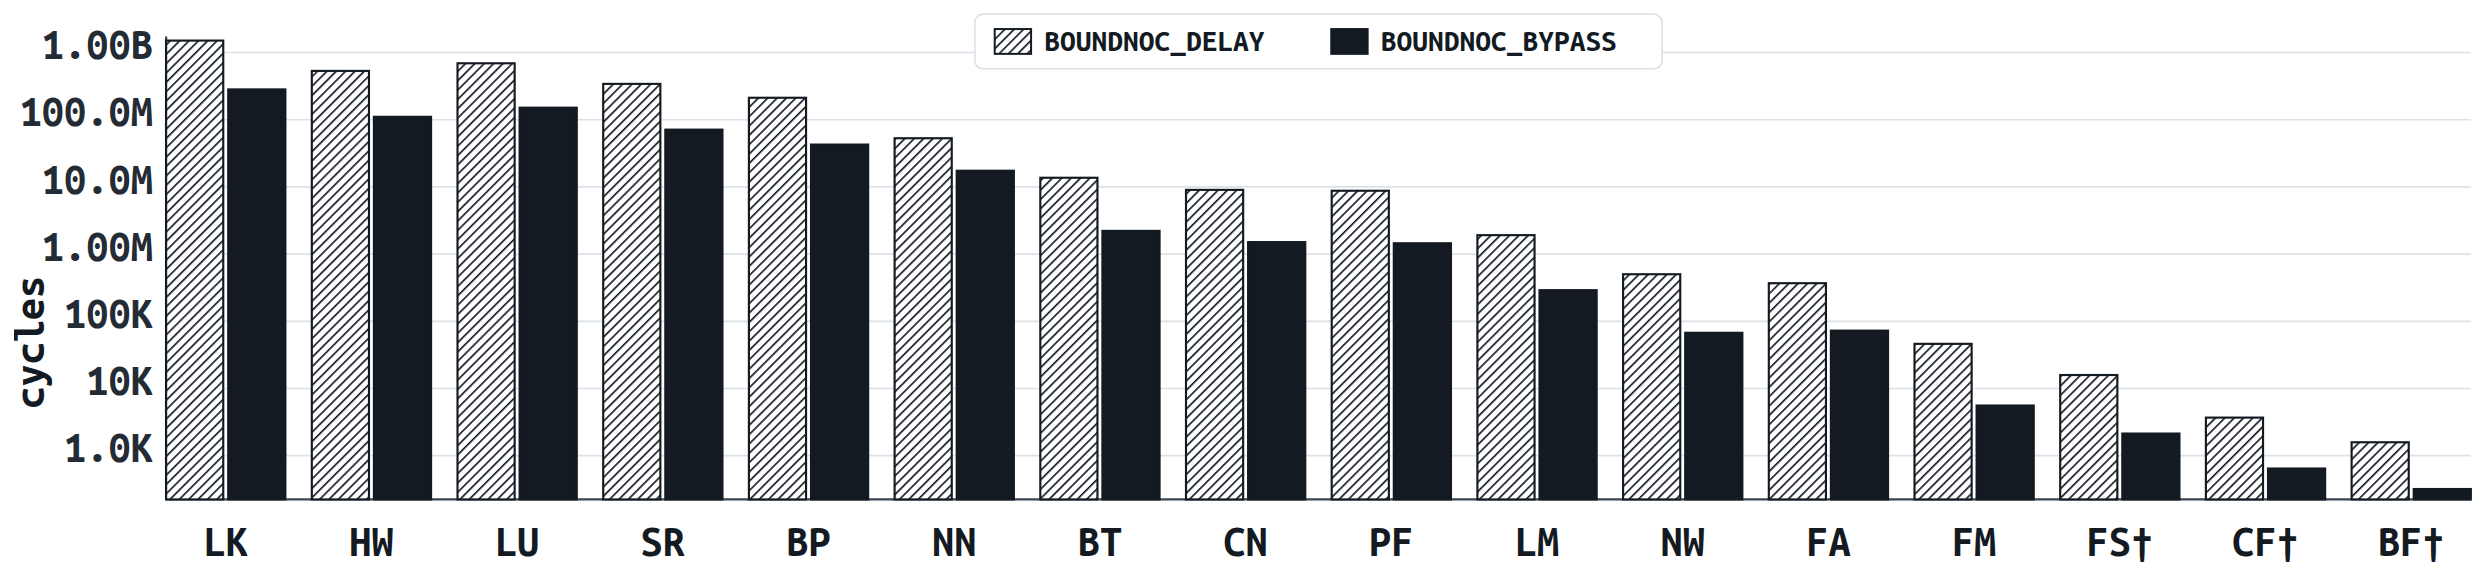
\includegraphics[width=\linewidth]{figs_new/boundnoc_delay_amount.png}
    %{figs/delay-amount.pdf}
    \caption{Total delay cycles accumulated in the delay queue for PARSEC applications under \jscheme{} and \bscheme{}.}
    \label{fig:delay-amount}
\end{figure*}

\subsection{MLPerf Overheads} \label{sec:mlperf}
We present the overheads of \jscheme{} and \bscheme{} on MLPerf TinyML~\cite{banbury2021mlperf} workloads in Figure~\ref{fig:impact-on-mlperf}.

\begin{figure}[t]
   \centering
    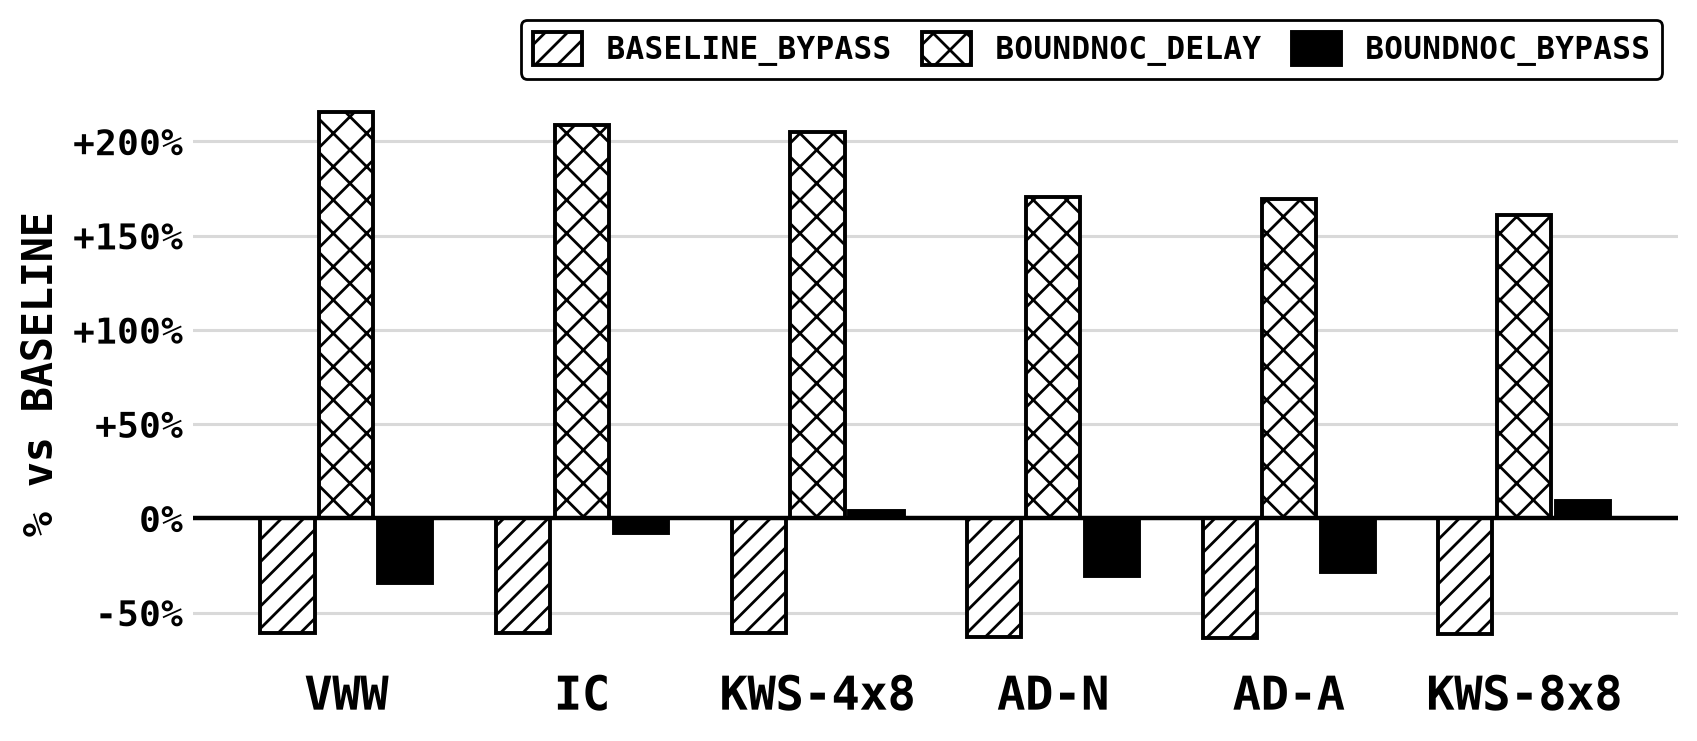
\includegraphics[width=\linewidth]{figs_new/boundnoc_ml_latency_pctdelta.png}
    %{figs/impact-on-latency.pdf}
    \caption{Mean attack-packet latency under \basebscheme{}, \jscheme{}, and \bscheme{}, expressed as \% change relative to \basescheme{}, for four MLPerf TinyML inference workloads. 
    KWS is shown at both a $4\times8$ and an $8\times8$ mesh to isolate topology effects; AD is shown for both its AD-N and AD-A input classes.}
    \label{fig:impact-on-mlperf}
\end{figure}

We evaluate four TinyML inference workloads from the MLPerf TinyML suite: Anomaly Detection (AD), Keyword Spotting (KWS), Image Classification (IC), and Visual Wake Words (VWW).
Each workload is a fully int8-quantized TensorFlow Lite Micro model, compiled into a statically-linked musl binary and executed natively on each simulated core.
No host-side interpretation or instrumentation is introduced into the timing loop.

AD uses a $270$~KB fully-connected deep autoencoder~\cite{autoencoder} over a 5-frame, 128-band log-mel spectrogram ($5\times128$) derived from the ToyADMOS industrial-sound dataset~\cite{koizumi2019toyadmos} to perform unsupervised anomaly detection.
It completes with $2.9$~million instructions per core. 
We evaluate both a \emph{normal} (AD-N --- a recording of the ToyCar operating normally) and an \emph{anomalous} (AD-A --- containing an injected mechanical fault) input clip, replicated across 64 independent instances on an $8\times8$ mesh.

KWS performs small-vocabulary keyword spotting with a $52.5$~KB depthwise-separable CNN (DS-CNN)~\cite{zhang2017hello} over a $49\times10$ MFCC feature matrix extracted from the Google Speech Commands dataset~\cite{warden2018speech}. 
It completes with $204$~million instructions per core -- an order of magnitude more compute-intensive than AD.
Because of this cost, we evaluate KWS at both a $4\times8$ mesh (32 instances, KWS-4x8) and the standard $8\times8$ mesh (64 instances, KWS-8x8) to separate topology effects from workload effects.

IC performs 10-class image classification with a $96$~KB ResNet8~\cite{he2016resnet} model over $32\times32\times3$ CIFAR-10~\cite{krizhevsky2009learning} images. 
It completes with $941$~million instructions per core, replicated across 32 instances on a $4\times8$ mesh.

VWW performs binary person detection with a $325$~KB, width-reduced ($0.25\times$) MobileNetV1~\cite{howard2017mobilenets} model over $96\times96\times3$ crops from the Visual Wake Words dataset~\cite{chowdhery2019vww}. 
It completes with $628$~million instructions per core, also replicated across 32 instances on a $4\times8$ mesh.

As with the Rodinia and PARSEC results in Section~\ref{sec:eval-setup}, we mark memory accesses of every core  as Security Sensitive to model the worst case, and use $T_{low}=50$ and $T_{worst}=100$ cycles for \bscheme{} and \jscheme{} respectively.
Because AD, IC, and VWW are single-threaded inference binaries, we replicate an independent instance to every core rather than let 63 cores sit idle waiting on a single active thread.

Figure~\ref{fig:impact-on-mlperf} shows the mean attack-packet latency under each policy, expressed as percentage change relative to \basescheme{}.
Across all six workload/mesh combinations, \basebscheme{} reduces mean attack-packet latency by $60\%$--$63\%$ and \jscheme{} increases it by $161\%$--$216\%$, consistent with the Rodinia/PARSEC results in Section~\ref{sec:perf-overhead}. 
\jscheme{} enforces the fixed worst-case latency $T_{worst}$ for every Security Sensitive access regardless of workload, while \basebscheme{} is bounded only by how much traffic the bypass path can absorb.

\bscheme{} shows a workload-dependent split not previously visible from Rodinia and PARSEC alone.
On AD-N, AD-A, and VWW, \bscheme{} closely tracks \basebscheme{}, improving over \basescheme{} by $30.5\%$, $28.7\%$, and $34.2\%$ respectively.
On KWS and IC, \bscheme{} instead lands close to or slightly above \basescheme{}: $+9.1\%$ on KWS-8x8, $+4.1\%$ on KWS-4x8, and $-8.0\%$ on IC.
The KWS regression is robust to topology -- it appears at both $4\times8$ and $8\times8$ mesh, ruling out mesh diameter as the sole cause. 
IC reproduces the same weak-to-negative pattern despite running on the same $4\times8$ mesh as VWW, which shows the opposite, favorable result.

We compared the bypass-eligible packet fraction, jittered-packet fraction, and mean hop count across all six runs and found no single aggregate statistic that cleanly separates the two groups.
Bypass-eligible fraction is nearly uniform ($62\%$--$71\%$) across all six. 
Jittered-packet fraction separates AD from KWS at matched $8\times8$ scale ($4.1\%$ vs.\ $18.3\%$) but not IC from VWW at $4\times8$ scale ($98.5\%$ vs.\ $67.3\%$, the wrong direction).
Mean hop count tracks mesh geometry rather than the workload grouping.

We conclude that the hop-count-based bypass eligibility threshold for \bscheme{} is not uniformly effective across all inference workloads. 
The convolutional, activation-heavy access patterns of KWS and IC appear less amenable to it than the single fully-connected pass of AD or the wider MobileNet of VWW. 
We leave a precise mechanistic explanation to future work; Section~\ref{sec:eval-rand} explores a different mitigation, randomizing the convergence target instead of the eligibility threshold itself.

\subsection{\rscheme{}: A Randomized-Target Alternative} \label{sec:eval-rand}
As a sensitivity study over the randomization window (Section~\ref{sec:eval-setup}), we compare \bscheme{} against two alternative target ranges.
\bscheme{} underperforms on two of the six MLPerf combinations: KWS-4x8 ($+4.1\%$) and KWS-8x8 ($+9.1\%$), with IC only a modest improvement ($-8.0\%$).
This motivates \rscheme{} (Section~\ref{sec-rscheme}), which draws a random target per access instead of the fixed $T_{low}$.

We first tried a wider variant (\rejscheme{}) that draws the target uniformly from $[T_{floor}, T_{worst}]$ instead of $[T_{floor}, T_{low}]$.
This wider range costs too much average latency in practice: it lands worse than \basescheme{} on every benchmark we tested.
We do not use it further.

\rscheme{} instead draws from the narrower $[T_{floor}, T_{low}]$ range.
Figure~\ref{fig:variable-workload} compares \basebscheme{}, \bscheme{}, \rejscheme{}, and \rscheme{} on eight benchmarks spanning MLPerf, PARSEC, and Rodinia.
\rscheme{} fixes both weak MLPerf cases -- IC improves to $-41.0\%$, KWS-4x8 to $-32.5\%$, KWS-8x8 to $-26.3\%$ -- while making the already-strong PARSEC and Rodinia cases stronger still.
\rscheme{} is a clean latency win on every benchmark tested.

\begin{figure*}[t]
\centering
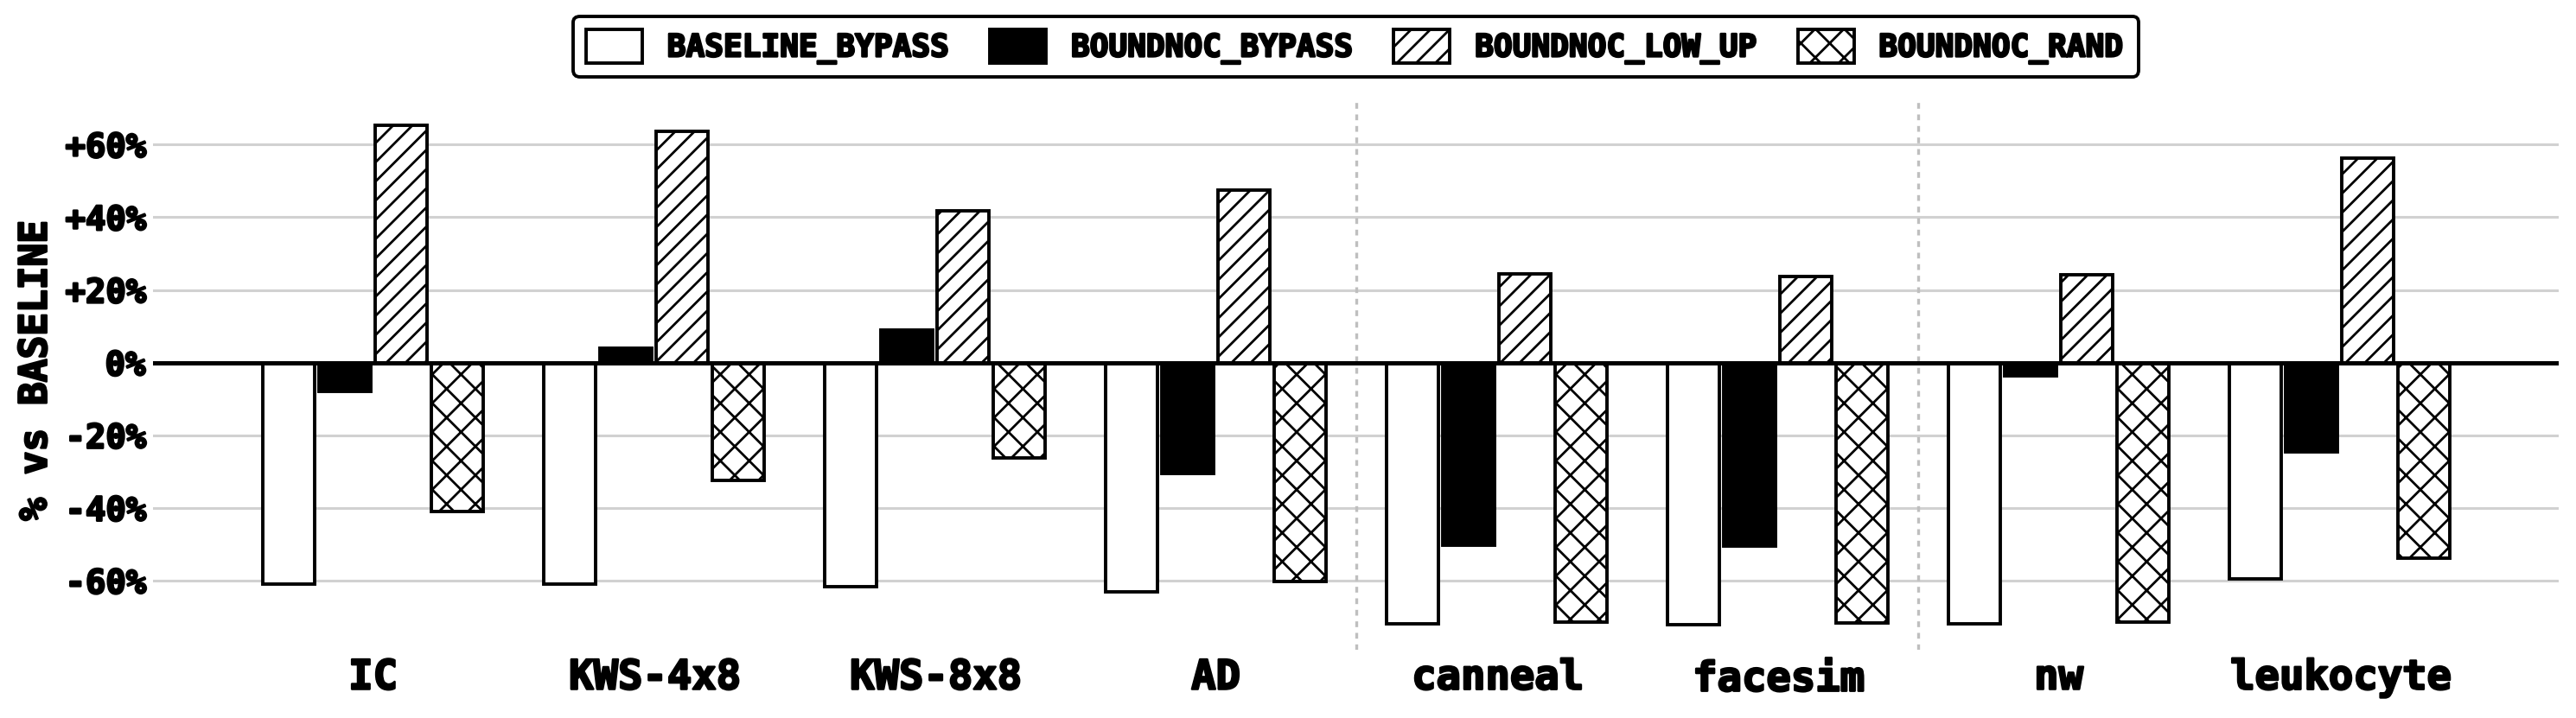
\includegraphics[width=\linewidth]{figs_new/boundnoc_variable_workload_pctdelta.png}
\caption{Mean attack-packet latency under \basebscheme{}, \bscheme{}, \rejscheme{}, and \rscheme{}, expressed as \% change relative to \basescheme{}, across eight benchmarks spanning MLPerf TinyML, PARSEC~\cite{bienia2008parsec}, and Rodinia~\cite{che2009rodinia}.}
\label{fig:variable-workload}
\end{figure*}

This latency benefit does not come with the same security guarantee as \bscheme{}, however.
Section~\ref{sec-security-rand} shows \rscheme{} is less effective than \bscheme{} at hiding distance, though still better than \basebscheme{}.

\subsection{Hardware Overhead} \label{sec:hw-overhead}
We estimate the hardware cost using CACTI-7~\cite{cacti} at 22~nm.
\scheme{} introduces minimal changes to both the NIs and the routers.
NI changes include a delay queue ($0.981~mm^{2}$, $0.028~nJ$/access) and 512 64-bit comparators.
An arbitration unit with two multiplexers is also added, with negligible area cost.
The bypass channel adds $2.34\%$--$4.69\%$ area overhead compared to a conventional NoC~\cite{ma2021latency}.

In summary, \bscheme{} provides the same security guarantees as \jscheme{} while incurring no performance overhead compared to \basescheme{} and minimal hardware cost.
\jscheme{} offers a simpler implementation at the cost of a $7.24\%$ average performance overhead.
